\documentclass[11pt,compress,t,notes=noshow, aspectratio=169, xcolor=table]{beamer}

\usepackage{../../style/lmu-lecture}
% Defines macros and environments
% This file is included in slides and exercises

% Rarely used fontstyle for R packages, used only in 
% - forests/slides-forests-benchmark.tex
% - exercises/single-exercises/methods_l_1.Rnw
% - slides/cart/attic/slides_extra_trees.Rnw
\newcommand{\pkg}[1]{{\fontseries{b}\selectfont #1}}

% Spacing helpers, used often (mostly in exercises for \dlz)
\newcommand{\lz}{\vspace{0.5cm}} % vertical space (used often in slides)
\newcommand{\dlz}{\vspace{1cm}}  % double vertical space (used often in exercises, never in slides)
\newcommand{\oneliner}[1] % Oneliner for important statements, used e.g. in iml, algods
{\begin{block}{}\begin{center}\begin{Large}#1\end{Large}\end{center}\end{block}}

% Don't know if this is used or needed, remove?
% textcolor that works in mathmode
% https://tex.stackexchange.com/a/261480
% Used e.g. in forests/slides-forests-bagging.tex
% [...] \textcolor{blue}{\tfrac{1}{M}\sum^M_{m} [...]
% \makeatletter
% \renewcommand*{\@textcolor}[3]{%
%   \protect\leavevmode
%   \begingroup
%     \color#1{#2}#3%
%   \endgroup
% }
% \makeatother


\newcommand{\pih}{\fh}

\title{Interpretable Machine Learning}
% \author{LMU}
%\institute{\href{https://compstat-lmu.github.io/lecture_iml/}{compstat-lmu.github.io/lecture\_iml}}
\date{}

\newcommand{\gh}{\hat{g}}

\begin{document}

	
% Set style/preamble.Rnw as parent.

% Load all R packages and set up knitr

% This file loads R packages, configures knitr options and sets preamble.Rnw as 
% parent file
% IF YOU MODIFY THIS, PLZ ALSO MODIFY setup.Rmd ACCORDINGLY...

% Defines macros and environments

\newcommand{\titlefigure}{figure/lime5}
\newcommand{\learninggoals}{
	\item Understand motivation for LIME
	\item Develop a mathematical intuition}

\lecturechapter{Local Interpretable Model-agnostic Explanations (LIME)}
\lecture{Interpretable Machine Learning}

% Prerequisite: le-intro

% ------------------------------------------------------------------------------
% \begin{frame}{LIME}
% \begin{itemize}
% 		% \item LIME assumption: Even if an ML model is very complex, local predictions may be explained by a simpler, interpretable model
% 		% \smallskip\pause
% 		\item LIME explains \textbf{individual} predictions of \textbf{any} black-box model by approximating the model \textbf{locally} with an interpretable model (local surrogate model)\\
%         $\leadsto$ \textbf{Assumption:} Complex models behave simply in small input neighborhoods
% 		\smallskip\pause
% 		\item Called local surrogate models $\leadsto$ often inherently interpretable models such as linear models or classification/regression trees are chosen\\
% 		\smallskip\pause
% 		\item LIME should answer why a ML model predicted $\hat y$ for input $\xv$
% 		\smallskip\pause
% 		\item LIME is model-agnostic and can handle tabular, image and text data 
% \end{itemize}
% \end{frame}

% Improved slide: LIME – Local Surrogate Explanations
\begin{frame}[t]{LIME}
  \begin{itemize}%[<+->]
    %\item \textbf{Key idea:} Approximate any black‑box model $\fh$ around a single input $\xv$ with an \emph{interpretable} surrogate $\gh$
    \item \textbf{Locality assumption:} $\fh$ behaves similarly simple in small neighborhood of $\xv$\\
    $\leadsto$ Approximate $\fh$ near $\xv$ using an interpretable surrogate model $\gh$
    \item \textbf{Interpretation strategy:} Use $\gh$'s simple internal structure to explain $\fh(\xv)$ locally\\
    $\leadsto$ \textbf{Common surrogates:} Sparse linear models, shallow decision trees
    %\item \textbf{Algorithm:} Perturb $\xv$, obtain $\fh(\tilde{\xv})$, weight by proximity, fit $\gh$ to weighted data, interpret $\gh$’s parameters
    %\item \textbf{Typical uses:} Debug single predictions, detect spurious features, provide actionable recourse
    \item \textbf{Applicability:} Model‑agnostic; supports tabular, image, and text data %via modality‑specific perturbations
    \item \textbf{In practice:} Generate samples near $\xv$, predict with $\fh$, and fit $\gh$ to these samples using $\fh$’s outputs as targets, weighting samples by their proximity/closeness to $\xv$

  \end{itemize}
\end{frame}


% \begin{frame}{LIME}
%   \begin{itemize}
%     \item<1-> \textbf{Core idea:} Complex models may be approximated locally by simpler, interpretable models\\
%     $\leadsto$ Explain individual predictions of any model via local surrogate models
%     \item<3-> \textbf{Surrogates:} Typically simple models (e.g., linear, decision tree) fitted to perturbed samples near the input $\xv$
%     \item<4-> \textbf{Goal:} Provide human-interpretable justification for why the model predicted $\hat{y}$ for input $\xv$
%     \item<5-> \textbf{Properties:} Model-agnostic; applicable to tabular, image, and text data (with modality-specific perturbations)
%   \end{itemize}
% \end{frame}


\begin{frame}{LIME: Characteristics}

    \textbf{Definition:}
	LIME provides a local explanation for a black-box model $\fh$ in form of a surrogate model $\gh \in \Gspace$, where $\Gspace$ is a class of interpretable models\\[2em]
	
	
	Surrogate model $\gh$ should satisfy two characteristics:
	\begin{enumerate}
		\item \textbf{Interpretable}: Provide human-understandable insights into the relationship between input features and prediction (e.g. via coefficients, model structure)
	\item \textbf{Local fidelity / faithfulness}: 
    $\gh$ closely approximates $\fh$ in the vicinity of the input $\xv$ being explained
        %similar behavior as $\fh$ in the vicinity of the obs. being predicted
	\end{enumerate}
	
	\vspace{2em}
	\textbf{Goal:} Find $\gh$ with \textbf{minimal complexity and maximal local fidelity} 
\end{frame}


\begin{frame}{Model Complexity}
    
    We can measure the complexity of $\gh \in \Gspace$ using a complexity measure $J: \mathcal{G} \to \R_{0}$ \lz % $J(\gh)$ \lz

 	\textbf{Example: (Sparse) Linear Models}\\
 	\begin{itemize}
 	    \item Let $\Gspace = \left\{g: \Xspace \to \R ~|~g(\xv) = s(\thetav^\top \xv)\right\}$ be the class of linear models
 	    \item $s(\cdot)$ is identity (linear model) or logistic sigmoid function  (logistic regression)
 	    \item[$\leadsto$] $J(g) = \sum_{j = 1}^p \ind_{\{ \theta_j \neq 0 \}}$: Count number of non-zero coefficients (via L$_0$-norm of $\thetav$)
 	\end{itemize}
 	\lz\pause
 	
 	\textbf{Example: Decision Trees}\\
 	\begin{itemize}
 	    \item Let $\Gspace = \left\{g:\Xspace \to \R ~|~g(\xv) = \sum_{m=1}^M c_m \ind_{\{ \xv \in Q_m \}}\right\}$ be the class of trees
        \item $Q_m$ are disjoint axis parallel regions (leaves) and $c_m \in \R$ constant predictions
        %\\ 	     i.e., the class of additive models (e.g., constant $c_m$)  over the leaf-rectangles $Q_m$
 	    \item[$\leadsto$] $J(g) = M$: Count number of terminal/leaf nodes
 	\end{itemize}
 	
\end{frame}
 
% \begin{frame}{Local model fidelity}
%  	\begin{itemize}
%  		\item $\gh$ is locally faithful to $\fh$ w.r.t. $\xv$ 
%  		if for $\zv \in \Zspace \subseteq \R^p$ close to $\xv$, predictions of $\gh(\zv)$ are close to $\fh(\zv)$ 
%  		\item In an optimization task: the closer $\zv$ is to $\xv$, the closer $\gh(\zv)$ should be to $\fh(\zv)$  
%  		\pause
%  		\item Two required measures:
%  		\begin{enumerate}
%  			\item A proximity (similarity) measure $\neigh(\zv)$ between $\zv$ and $\xv$, e.g. the exponential kernel:
%  			$$\neigh(\zv) = exp(-d(\xv, \zv)^2/\sigma^2)$$ 
%  			with $\sigma$ as the kernel width and $d$ as the Euclidean distance (numeric features) or the Gower distance (mixed features) 
%  			\pause
%  			\item A distance measure or loss function $L(\fh(\zv), \gh(\zv))$, e.g. the L$_2$ loss/squared error
%  			$$L(\fh(\zv), \gh(\zv)) = (\gh(\zv) - \fh(\zv))^2$$ 
%  		\end{enumerate}
%  		\pause
%  		\item Given points $\zv$, we can measure local fidelity of $\gh$ with respect to $\fh$ in terms of a weighted loss
%  		$$ L(\fh, g, \neigh) = \sum_{\zv \in \Zspace} \neigh(\zv) L(\fh(\zv), \gh(\zv)) $$
%  		%\item Note that identifying \textbf{locally} faithful explanations that are interpretable is less of a challenge than identifying \textbf{globally} faithful explanations. Yet, global fidelity implies local fidelity but not vice versa.
%  	\end{itemize}
% \end{frame}

\begin{frame}{Local Fidelity of Surrogate Models}

  \begin{itemize}
    \item Surrogate \( \gh \) is \textbf{locally faithful} to a black-box model \( \fh \) around an input \( \xv \) if
    \[
    \gh(\zv) \approx \fh(\zv) \quad \text{for synthetic samples } \zv \in \Zspace \subseteq \R^p \text{ generated around } \xv
    \]

    \pause

    \item \textbf{Optimization principle:} The closer \( \zv \) is to \( \xv \), the more \( \gh(\zv) \) should match \( \fh(\zv) \)

    \pause

    \item To operationalize this optimization, we need:
    \begin{enumerate}
      \item \textbf{A proximity (similarity) measure} $\neigh(\zv)$ between $\zv$ and $\xv$, e.g.:
      
        \medskip
        \centerline{$
        \neigh(\zv) = \exp(-d(\xv, \zv)^2 / \sigma^2)  \text{ (exponential kernel), where}
        $}
        \medskip
        
        \begin{itemize}
            \item \( d \) is a distance metric (e.g., Euclidean or Gower for mixed types)
            \item \( \sigma \) is the kernel width that controls locality
        \end{itemize}
        
        %(e.g., Euclidean or Gower), 
        

      \pause
      \item \textbf{A loss function} \( L(\fh(\zv), \gh(\zv)) \), e.g. the L$_2$ loss/squared error:
        \[
        L(\fh(\zv), \gh(\zv)) = \left( \gh(\zv) - \fh(\zv) \right)^2
        \]
    \end{enumerate}

    \pause

    \item The overall \textbf{local fidelity objective} is measured by a weighted loss:
    \[
    L(\fh, \gh, \neigh) = \sum_{\zv \in \Zspace} \neigh(\zv) \cdot L(\fh(\zv), \gh(\zv))
    \]
  \end{itemize}
\end{frame}







\begin{frame}{LIME Optimization Task}
	\begin{itemize}
		\item Optimization problem of LIME: 
		$$ \argmin_{\gh \in \Gspace} L(\fh, \gh, \neigh) + J(\gh)$$
		\item \textbf{In practice} LIME uses a two-stage approach:
		\begin{enumerate}
                \item User specifies complexity $J(\gh)$ beforehand (e.g., LASSO with \( k \) features)
		    \item Optimize $L(\fh, \gh, \neigh)$ (model fidelity) for fixed complexity
		\end{enumerate}
		\item \textbf{Goal:} Build a \textbf{model-agnostic} explainer
		\begin{itemize}
    		\item[$\leadsto$] Optimize $L(\fh, \gh, \neigh)$ without making any assumptions on the form of $\fh$ 
    		\item[$\leadsto$] Surrogate \( \gh \) approximates \( \fh \) locally through sampling and fitting
            %learn $\gh$ only approximately  
		\end{itemize}
		\end{itemize}
\end{frame} 

\begin{frame}{LIME Algorithm: Outline \citebutton{Ribeiro. 2016}{https://github.com/marcotcr/lime}}
		
		\textbf{Input}:
		\begin{itemize}
		    \item Pre-trained black-box model $\fh$
		    \item Observation $\xv$ whose prediction $\fh(\xv)$ we want to explain
		    \item Interpretable model class $\Gspace$ for local surrogate (to limit complexity)
		\end{itemize}
		
		\pause
		\medskip
		
		\textbf{Algorithm}:
		\begin{enumerate}
    		\item Independently sample new points $\zv \in \Zspace$ 
    		\item Retrieve predictions $\fh(\zv)$ for obtained points $\zv$ 
    		\item Weight $\zv \in \Zspace$ by their proximity $\neigh(\zv)$ to quantify closeness to \( \xv \)
    		\item Train interpretable surrogate model $\gh$ on data points $\zv \in \Zspace$ using weights $\neigh(\zv)$\\ $\leadsto$ Predictions $\fh(\zv)$ are used as target of this model
    		\item Return \( \gh \) as the local explanation for \( \fh(\xv) \)
            %the interpretable model $\gh$ as the explainer
		\end{enumerate}
		

	
\end{frame} 

\begin{frame}{LIME Algorithm: Example}

    	\textbf{Illustration} of LIME based on a classification task:
		\begin{itemize}
			\item Light/dark gray background: prediction surface of a classifier
			\item Yellow point: $\xv$ to be explained
			\item $\Gspace$: class of logistic regression models 
		\end{itemize}
		\begin{center}
			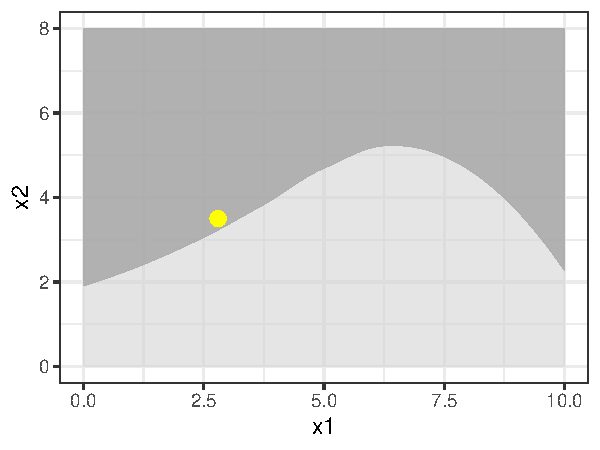
\includegraphics[width=0.6\textwidth]{figure/lime2}
		\end{center}

\end{frame} 


\begin{frame}{LIME Algorithm: Example (Step 1+2: Sampling)}
		
		Strategies for sampling: 
		\begin{itemize} 
			\item Uniformly sample new points from the feasible feature range 
			\item Use the training data set with or without perturbations
			\item Draw samples from the estimated univariate distribution of each feature
			\item Create an equidistant grid over the supported feature range  
		\end{itemize}
		\vspace{-.5cm}
		\begin{columns}[totalwidth=\textwidth]
        \begin{column}{0.5\textwidth}  %%<--- here
            \begin{figure}
             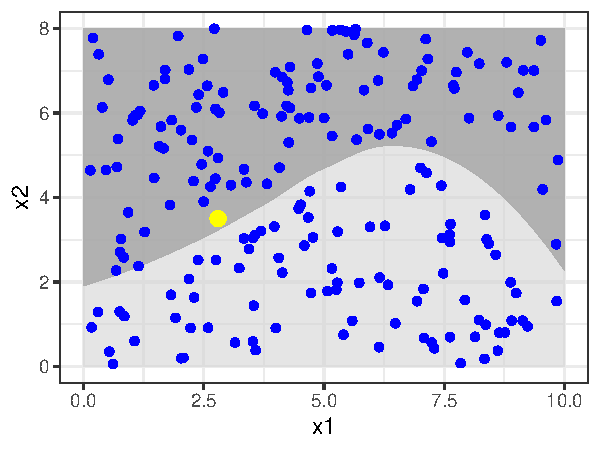
\includegraphics[width=.95\textwidth]{figure/lime3} 
             \vspace{-0.3cm}
             \caption{Uniformly sampled}
             \end{figure}
        \end{column}
        \begin{column}{0.5\textwidth}  %%<--- here
		    \begin{figure}
			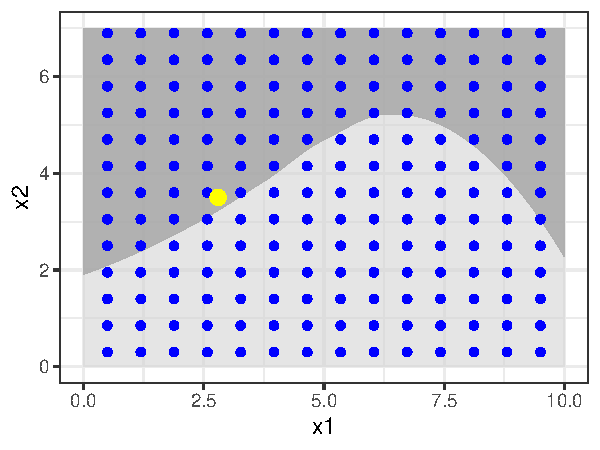
\includegraphics[width=.95\textwidth]{figure/lime3a}
			  \vspace{-0.3cm}
    		    \caption{Equidistant grid}
    		\end{figure}   
    \end{column}
\end{columns}
\end{frame}
		
\begin{frame}{LIME Algorithm: Example (Step 3: Proximity)}

	In this example, we use the exponential kernel defined on the Euclidean distance $d$
		 $$\neigh(\zv) = exp(-d(\xv, \zv)^2/\sigma^2).$$ 
		\begin{center}
			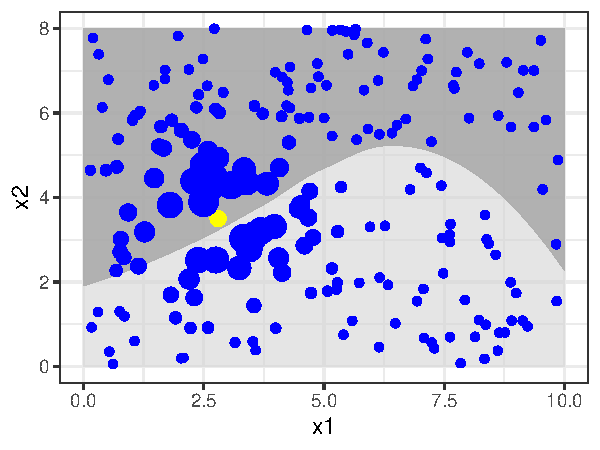
\includegraphics[width=0.7\textwidth]{figure/lime4}
		\end{center}
		
% MARIUS: Not relevant for the example; if we want to introduce it, we should do it somewhere else
% 	An alternative is the Gower proximity: 
% 	$\neigh(\zv) = 1 - \Gower(\zv, \xv) =  1 - \frac{1}{p}\sum_{j = 1}^{p} \delta_G(z_j, x_j) $ 
% 	$\textnormal{ with } \delta_G(z_j, x_j) = 
% 	\begin{cases}
% 	\frac{1}{\widehat{R}_j}|z_j- x_j| & \text{if $x_j$ and $z_j$ are numerical} \\
% 	\mathbb{I}_{z_j \neq x_j} & \text{if $x_j$ and $z_j$ are categorical}
% 	\end{cases}.$
		
\end{frame}
		
\begin{frame}{LIME Algorithm: Example (Step 4: Surrogate)}
		In this example, we fit a \textbf{logistic regression} model\\
        $\leadsto$ $L(\fh(\zv), \gh(\zv))$ is the Bernoulli loss
		\begin{center}
			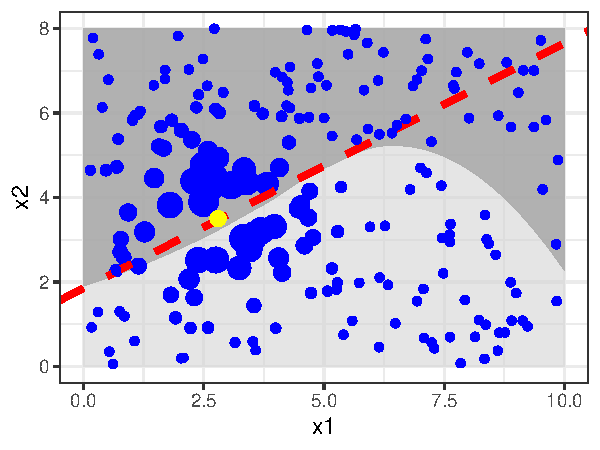
\includegraphics[width=0.7\textwidth]{figure/lime5}
		\end{center}
\end{frame}

\endlecture
\end{document}
